\chapter{The Comparative Study}
\label{chap:Comparative_Study}

This chapter provides the gui


This chapter provides the experiments and the results of this comparative study of countermeasures. As aforementioned in the last chapter, four countermeasures were selected and each one deal with one of the main cues mentioned in Section \ref{sec:SpoofingAttacksFaceRec} (liveness detection, scene characteristics and differences in image quality assessment). The countermeasures are:



\section{Evaluated countermeasures}
\label{sec:Evaluated_countermeasures}

For this comparative study were selected four countermeasures that do not depend of the user collaboration. Very representative according to the state of the art in the face antispoofing research, each one explore one of the main cues mentioned in the\ref{sec:SpoofingAttacksFaceRec}. Next subsections presents the details of each countermeasure and how was set each hyper-parameters of each one.

\subsection{Motion Correlation}

As presented in Section \ref{sec:scene_cues}, the Motion correlation \cite{AnjosIJCB2011} countermeasure measures the correlation between the face and it background. With some contributions by our side, the source code of this countermeasure is freely available \footnote{https://github.com/bioidiap/antispoofing.motion/}. There are, basically, two hyper-parameters in this countermeasure. The first one is the number of frames used to compute the 5 quantities. The second one is the binary classifier.

As the authors suggested, twenty frames to compute the 5 quantities are sufficient to the algorithm converge in their experiments. The classifier suggested in the paper was one based on Multi-layer Perceptron. This classifier has, basically, the number of hidden layers and the number neurons in each hidden layer as hyper-parameters. The authors suggested one hidden layer and five neurons in this hidden layer as good tradeoff between computational complexity and performance. 

\subsection{Textures with $LBP$}

Presented in Section \ref{sec:quality_assessment}, the countermeasure based on Textures with $LBP$ \cite{ChingovskaBIOSIG2012} and \cite{maatta2011face} explore the differences in texture properties between real accesses and attacks in single frames. 

There are, basically, three hyper-parameters in this countermeasure. The first one is the geometrically normalized face size. The authors suggested a face size of $64 \times 64$ pixels. The second one is the configuration of the $LBP$ texture descriptor. The $LBP$ itself has several hyper-parameters \ref{inen2011computer} and the authors of both papers stressed only some of that. In this thesis we will follow the setup suggested by \cite{ChingovskaBIOSIG2012} using the $LBP_{8,1}^{u2}$. Finally the last hyper-parameter is the binary classifier. The best classifier tested by \cite{ChingovskaBIOSIG2012} was the Support Vector Machines (SVM) using the Radial Basis Function (RBF). For this classifier the parameter $C$ (the cost of the loss function) and the $\gamma$ parameter (the variance of the radial function) was set to $1$ and $0.1$ respectively.

\subsection{Dynamic Textures with $LBP-TOP$}

Presented in the Chapter \ref{chap:Proposed_Countermeasures}, the countermeasure based on dynamic textures with $LBP-TOP$, explore the texture dynamics to detect attacks in a frame sequence. There are, basically, three hyper-parameters in this countermeasure. The first one is the geometrically normalized face size. In the last chapter, we worked with face sizes of $64 \times 64$ pixels and we are keep this in the next experiments. The second hyper-parameter is the configuration of the $LBP-TOP$ descriptor. As in the $LBP$, the $LBP-TOP$ descriptor itself has several hyper-parameters and each one was extensively tuned in the last chapter. As good tradeoff between computational complexity and performance we selected the following configuration: $LBP-TOP^{u2}_{8,8,8,1,1,1}$. The last hyper-parameter is the binary classifier. The evaluation method proposed in the last chapter suggested the SVM classifier with RBF kernel.


\subsection{Eye blinks}

The eye blink countermeasure used in this thesis uses a similar technique applied in Motion Correlation countermeasure\cite{AnjosIJCB2011}. The difference is; the accumulated motion $M_D$, (see Equation \ref{eq:motion}) is computed between the face region and the eyes region as can be observed in the Figure \ref{fig:eye_blink}. 

\begin{figure}[!btb]
\begin{center}
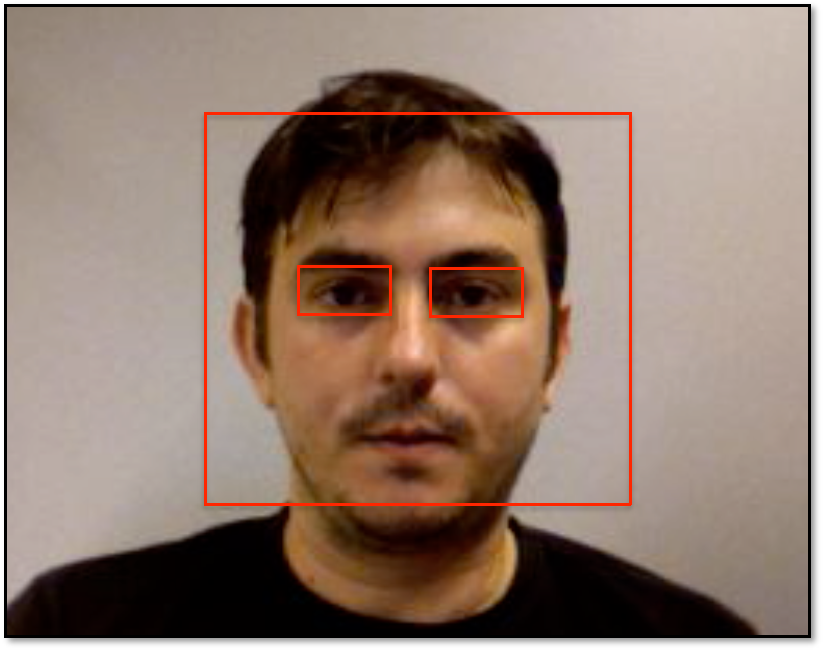
\includegraphics [width=10cm] {images/eye_blink.pdf}
\caption[Eye blink countermeasure scheme]{Eye blink countermeasure scheme}
\label{fig:eye_blink}
\end{center}
\end{figure}


The score for each single frame $n$ in a frame sequence, is computed using the following equation:
\begin{equation}
S_n=   \frac{M_{D_{eye}}(n)}{M_{D_{face}}(n)} - ravg(\frac{M_{D_{eye}}}{M_{D_{face}}})(n)
\label{eq:score_blink}
\end{equation}
where the $ravg$ is the remainder average in a frame sequence until the frame $n$.


\section{Evaluation method}
\label{sec:Evaluation_Protocol}

For this comparative study, we will evaluate the intra-database and the inter-database (or cross-database) generalization. For that, we developed two test protocols, the intra-test protocol and the inter-test protocol. 

The intra-test protocol evaluates the intra-database generalization. It consists in training, tuning and testing a countermeasure with the respectively training set, development set and test set of one database.

The inter-test protocol is a little bit more challenging since test the inter-database generalization (or cross-database). It consists in training and tuning a countermeasure with the training set and development set of one database and test it with the test set of others databases. 


%Firstly, we study how the countermeasures, presented in Section \ref{sec:countermeasures}, will perform in a more realistic condition. This condition consists in training and tuning each one of the countermeasures with one face anti-spoofing database and testing with another one. To report the performance in such a scenario, two evaluation protocols were designed to work with the databases described in Section \ref{sec_replay}. These protocols are the "intra-test" protocol and the "inter-test" protocol.


%The inter-test protocol evaluates the countermeasure performance in a more realistic scenario, close to real usage conditions. It consists in training and tuning a countermeasure with the training set and development set of one database and test it with the test set of another one. With this protocol, it is possible to evaluate the performance and the generalization power of a countermeasure in a set of unseen types of attacks.


\section{Evaluation Metrics}

The final performance of each countermeasure using both evaluation protocols in the test set of each database is reported with the Half Total Error Rate ($HTER$): 

\begin{equation}
\label{eq:HTER}
HTER(D_2)=\frac{FAR(\tau(D_1),D_2)+ FRR(\tau(D_1),D_2)} {2} ,
\end{equation}
where $\tau(D_n)$ is the decision threshold, $D_n$ is the dataset, $FAR$ is the False Acceptance Rate in the database $D_2$ and $FRR$ is the False Rejection Rate in the database $D_2$. In this protocol, the value of $\tau(D_n)$ is estimated on the Equal Error Rate (EER) using the development set of the database $D_1$. 

In this equation, to measure the performance using the intra-database protocol, is necessary to consider $D_1 = D_2$. To measure the performance using the inter-database protocol, is necessary to make $D_1 \neq D_2$.


\section{Evaluated data}

As the Motion correlation, $LBP-TOP$ and the eye blink countermeasures need a frame sequence to work, the databases evaluated in this dissertation will be the Replay Attack Database (Section \ref{sec_replay}) and CASIA Face Antispoofing Database (Section \ref{sec_casia}).

As already mentioned in Section \ref{sec_replay} the Replay Attack Database has three non-overlapping partitions; the training, development and test set for respectively train, tune and test a countermeasure. To run the proposed protocols in this database, we will used the train set to train the four countermeasures; the development set will be used to estimate the value of $\tau(D_1)$. Finally the test set will be used to report the $HTER(D_2)$.

The CASIA FASD lacks a specific development set; this database has only a train and a test set. Since we need the three sets (train, development and test), we split the train set in five partitions and a 5-fold cross-validation training was done. For that, 4 folds were used for training and 1 fold was used to estimate the value of $\tau(D_1)$. The original test set was preserved, to report the $HTER(D_2)$. Because of 5-fold cross validation protocol, for the CASIA FASD 5 results were generated. The average of $HTER$ was provided as a final result.


